\title{Evaluating Performance of Anti-Entropy Algorithms}
\author{Kenny Gao\\Sriram Mohan, Advisor\\Rose-Hulman Institute of Technology }
\date{\today}

\documentclass[11pt,letterpaper]{article}
\usepackage[latin1]{inputenc}
\usepackage{amsmath}
\usepackage{amsfonts}
\usepackage{amssymb}
\usepackage{graphicx}
\usepackage[parfill]{parskip}
\linespread{1.1}

\begin{document}
\maketitle

\newpage 

\begin{abstract}
Distributed databases circumvent numerous performance issues presented by traditional databases, but introduce inherent limitations of their own - Brewer's CAP theorem states that a distributed system cannot guarantee all three properties of consistency, availability, and partition tolerance at the same time. This typically results in consistency being scaled back to the weaker eventual consistency. In order to enforce eventual consistency in a system containing replicated data, distributed databases like Amazon's Dynamo and Apache Cassandra make use of a process called anti-entropy, implemented using Merkle trees. Here, I evaluate the performance of Merkle tree-based anti-entropy and look at ways in which it can be improved.
\end{abstract}

\newpage 

\tableofcontents

\newpage 

\section{Introduction}
As software makes its transition from the desktop to the web, distributed databases have emerged as a popular solution to handle the issues presented by the need to provide functionality at scale. The high availability and tolerance for network partitions that they provide, however, comes with the cost of weakened consistency, as shown to be necessary by Brewer's CAP theorem\cite{Brewer:2000:TRD:343477.343502}. In order to accommodate this limitation, distributed databases implement a suite of consistency-providing techniques. One such technique is called anti-entropy, and is implemented via the use of Merkle trees\cite{Merkle:1987:DSB:646752.704751}.

In this paper, we'll begin by elaborating upon the context behind Merkle tree-based anti-entropy in greater detail. From there, we'll delve into the motivation behind evaluating the performance of anti-entropy algorithms. Then, we'll establish what performance is and what algorithms to evaluate, describe the approach to and the implementation of the algorithm simulation framework, and review the resultant data. Finally, we'll extrapolate some implications from the results and discuss avenues for further work on this topic.

\section{Background}

\subsection{Distributed Databases}
A distributed database is a database in which data is held in multiple physical locations. Examples include Google's BigTable\cite{Chang:2008:BDS:1365815.1365816}, Amazon's Dynamo\cite{DeCandia:2007:DAH:1323293.1294281}, and Apache Cassandra\cite{Lakshman:2010:CDS:1773912.1773922}.

\subsection{The CAP Theorem}
Eric Brewer's CAP theorem states that a distributed database cannot guarantee all three properties of consistency, availability, and partition tolerance at the same time.

\subsection{Eventual Consistency}
As a result, modern distributed databases are designed to guarantee only availability and partition tolerance. Consistency, on the other hand, is replaced with the weaker eventual consistency\cite{Vogels:2009:EC:1435417.1435432}, which allows data to be inconsistent across replicas with the understanding that conflicts will eventually be resolved.

\subsection{The Need for Anti-Entropy}
Techniques like read-repair, write-repair, and hinted handoff cover most conflict resolution cases - particularly, those caused by minor replica failures. To resolve prolonged replica failures, distributed databases rely on a technique called anti-entropy. When a replica that has experienced prolonged failure rejoins the system, anti-entropy synchronizes its data with that of another replica, resolving the conflicts between the two. Without it, we would be forced to choose between slowing down I/O (read/write-repair), re-instancing the replica, or using another asynchronous conflict resolution method.

\subsection{Merkle Trees}
Distributed databases such as Dynamo and Cassandra implement anti-entropy using Merkle trees, or hash trees. Merkle trees are trees of hashes in which parent nodes hold the hash of the concatenation of the hashes of their children, and the leaf nodes are hashes of some array of data.

\section{Motivation}
Although there was a reasonable amount of literature describing the role and function of Merkle trees in anti-entropy schemes, there was a distinct lack of justification for using them. With even a basic understanding of how they function, it cannot be denied that Merkle trees perform their duty adequately, but as I read more and more, I wondered: \textit{Why are they the best choice?} To answer that question, I first needed to answer the more immediate one of \textit{Exactly how ``good'' are Merkle trees?}

Of course, both questions are vague and unanswerable without first establishing some definitions and context. The key concept that needs to be disambiguated is that of performance. What exactly does ``good'' mean?

\section{What Performance is}
There are a number of ways for us to define performance, and each have merits. A sample of them are listed below.

\begin{itemize}
\item \textbf{Speed (time)} - At first glance, this is the option that stands out as the most obvious. Ultimately, speed is king, but it's also difficult to measure reliably. Speed is the final result of countless variables that factor into performance, including both those which stem from theory and those which stem from implementation. Existing literature describing the implementation of Merkle trees in anti-entropy schemes reveal heavy usage of caching, lazy tree generation, and amortization of initial costs, and while those techniques are important, they reveal little of the intrinsic performance of Merkle trees.

\item \textbf{Network usage} - An argument can be made that the real cost of anti-entropy is not experienced by the replicas themselves, but by the connections between them. Network usage is also largely unaffected by the implementation-level optimizations mentioned previously, as they operate exclusively within the replicas and have no bearing on the communication between replicas. As an additional bonus, network usage is fairly straightforward to measure via simulation.

\item \textbf{Qualitative criteria} - Undeniably, there are both advantages and disadvantages to using Merkle trees that can't be quantitatively measured. One such advantage, mentioned above, is its conduciveness to optimization at the implementation level with techniques such as caching, lazy tree generation, and amortization of initial costs. Not all techniques can be optimized in this way, and as such, it may be serve as a major differentiating factor between it and other anti-entropy techniques. Unfortunately, ``ease of optimization'' is not something that can be quantitatively measured.
\end{itemize}

After careful consideration, I chose network usage as the main criterion of evaluation. Its ease of measurement via simulation and its representation of a key component of anti-entropy performance made my goal of evaluating said performance both within reach and meaningful.

\section{What to Evaluate}
Having established network usage as the measurement criterion, we need to decide what we will be applying measurement to. That is, what algorithms are we interested in comparing the standard Merkle tree algorithm to?

A comparison study like this one requires adequate context in the form of a baseline to compare everything to. That is, we require, at the minimum, a base case algorithm to compare all other algorithms to. In the context of anti-entropy, that base case algorithm will be the one in which \textit{Replica A} sends its entire dataset to \textit{Replica B}, and \textit{Replica B} informs \textit{Replica A} of the values that require updating.

It may also be worth looking at variations on the standard Merkle tree algorithm. Specifically, we can fill in the gamut between the base case algorithm and the standard Merkle tree algorithm with algorithms that construct partial trees of varying depth. Additionally, we can look in orthogonal directions at ways to change components of the standard Merkle tree algorithm to optimize for certain inputs or cases.

To put all of these ideas into concrete examples, we could look at the following set of algorithms:

\begin{itemize}
\item Pairwise data comparison (naive)
\item Naive algorithm with single hash of all data
\item Naive algorithm with multiple layers of hashing
\item Standard Merkle tree algorithm (full hash tree)
\item Variations: non-binary trees, short-circuiting with base case failover
\end{itemize}

\section{Approach}
One of the key benefits of choosing network usage as the criterion of performance is its ease of measurement via simulation. We take full advantage of that fact in planning our approach.

\begin{quote}
Given the following variables:
\begin{itemize}
\item \# of data items stored on replicas
\item \# of conflicts between replicas
\end{itemize}
Measure each algorithm's performance in terms of network usage.

Repeatedly simulate on randomly-generated data for each configuration of variables.
\end{quote}

\section{Implementation}
The simulation framework is written in Python 2.7 and runs 100 independent simulations, for each configuration of variables, for both the naive algorithm and the standard Merkle tree algorithm, using randomly generated data.

The number of data items stored on replicas (\textit{datacount}) was set to 16 and 32. Setting \textit{datacount} to 64 (the simulation framework assumed that \textit{datacount} was a power of two) led to prohibitively-long simulation times.

The number of conflicts between replicas (\textit{conflictcount}) was set to values from 1 to \textit{datacount}, inclusive.

\section{Results}
\begin{figure}[hbtp]
\caption{network usage for \textit{datacount} = 16}
\centering
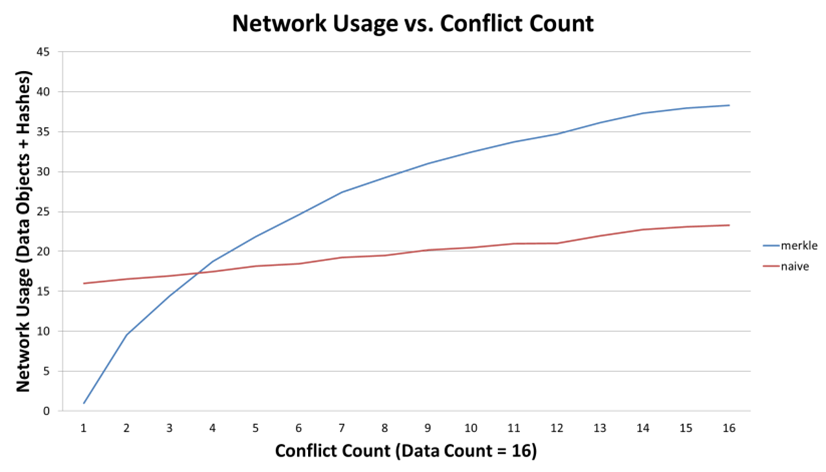
\includegraphics[scale=0.7]{results16.png} 
\end{figure}

\begin{figure}[hbtp]
\caption{network usage for \textit{datacount} = 32}
\centering
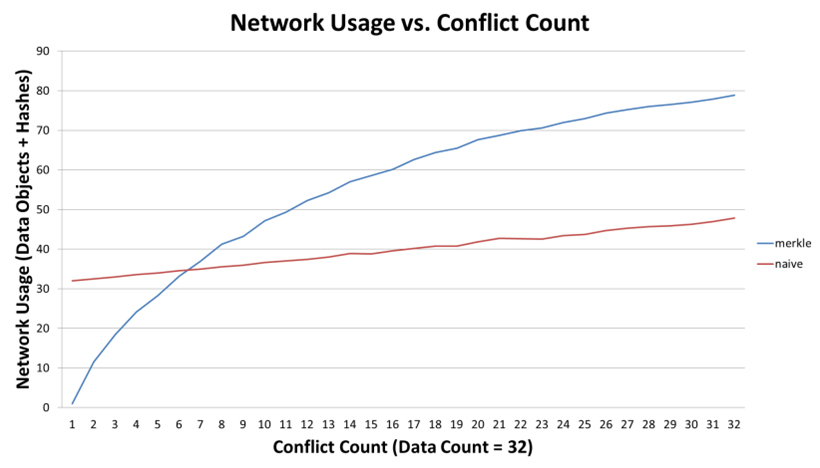
\includegraphics[scale=0.7]{results32.png} 
\end{figure}

Interestingly, we see that while the standard Merkle tree algorithm outperforms the naive algorithm when \textit{conflictcount} is low, the reverse is true when \textit{conflictcount} is high. The break-even point for \textit{conflictcount} is at only around 22\% of \textit{datacount}. We see this behavior for both \textit{conflictcount} = 16 and \textit{conflictcount} = 32.

In addition, we notice that the naive algorithm grows linearly with respect to \textit{conflictcount} (predictably, given the nature of the algorithm), whereas the standard Merkle tree algorithm grows approximately logarithmically. Again, we see this behavior for both \textit{conflictcount} = 16 and \textit{conflictcount} = 32.

Due to computational limitations, we must assume that these results do scale with respect to \textit{conflictcount}.

\section{Implications}
The most immediate implication is that the standard Merkle tree algorithm is indeed not the ``best'' in terms of network usage in all circumstances. In fact, it loses to the naive base case algorithm for \textit{conflictcount} $ > $ 22\% of \textit{datacount}! We now have evidence that different algorithms may be ``best'' at different points on the \textit{conflictcount} spectrum.

From the above, it follows that current anti-entropy methods could be improved by estimating the \textit{conflictcount} of replica pairs. Given the performance profiles of a set of algorithms with respect to \textit{conflictcount} and an estimated value for \textit{conflictcount}, we can always pick the algorithm with the best performance for that particular value.

It should be reiterated, however, that these results are, by design, only concerned with network usage. Other criteria for performance may be equally or more important in various circumstances, and are not represented by these results.

It's also worth noting that we only considered \textit{conflictcount} as our independent variable; other properties such as the spacial locality of the conflicts may also factor into performance.

\section{Further Work}
\subsection{Implement remaining algorithms}
Implementing and simulating the remaining algorithms in the list presented earlier would serve as a very reasonable next step. Perhaps we'd find that the standard Merkle tree algorithm is not the ``best'' in terms of network usage for any value of \textit{conflictcount}. Or, perhaps we'll discover the opposite, giving credence to the widespread usage of the algorithm.

\subsection{Extend performance evaluation}
Also worth exploring are ways to evaluate performance other than network usage. We discussed some of these alternatives earlier, but it was certainly not an exhaustive discussion. Establishing multiple criteria for performance would yield a more nuanced perspective on how ``good'' the algorithms are in relation to one another.

\subsection{Investigate other variables that might impact performance}
We only considered \textit{conflictcount} as an independent variable, but it's certainly not the only valid choice. Intuitively, the structure of Merkle trees would favor datasets in which conflicts were grouped together and wound up being represented in the same Merkle subtree. Certainly, the algorithm could be enhanced to take advantage of such cases. Thus, the spacial locality of the conflicts between datasets could be an important variable to consider when evaluating anti-entropy algorithm performance.

\newpage 

\bibliographystyle{plain} 
\bibliography{paper}

\end{document}